\chapter{MobiTrade: Implementation on Android Platform}
\label{chapter:MobiTrade}
\minitoc

We present in this chapter the design of the MobiTrade application for opportunistic collaborative content sharing that we have implemented for the android platform. We follow a top-down description approach. So, we start by giving a high level overview of the MobiTrade application architecture and its design principles in Section~\ref{MobiTradeArchitecture} namely MobiTrade functional blocks, followed by a description of the mobile application architecture and the content sharing session. Then, we dig deeper into the network and link level technical details of the MobiTrade android application in Section~\ref{MobiTradeDesignAndImplementation}. In Section~\ref{MobiTradeCurrentFunctionalities}, we describe through screen shots the set of functionalities actually provided. Finally, we conclude this chapter with a discussion of the open issues and a summary in Section~\ref{MobiTradeSoftSummary}.

\section{MobiTrade Architecture Overview}
\label{MobiTradeArchitecture}

\subsection{MobiTrade Functional Architecture}
\label{MobiTrade-functional-architecture}

Having described MobiTrade algorithms in chapter~\ref{chapter:PTMP}, we give here some more details of the MobiTrade functional architecture that encapsulates the latter algorithms. Figure~\ref{MobiTrade-node-architecture} is a schematic of MobiTrade functional architecture which encapsulates 5 building blocks:

\begin{figure}[!h]
\centering
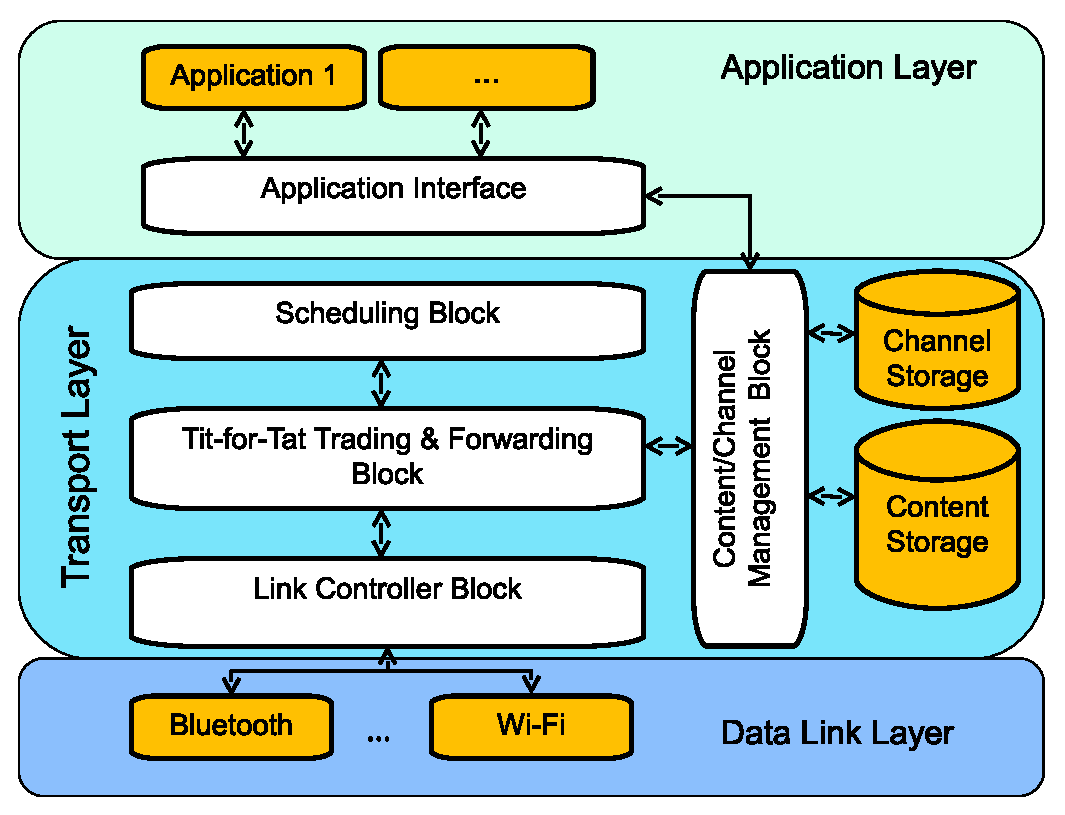
\includegraphics[width=3.5in,height=3in]{Chapitre6/MobiTrade_Node.eps}
\vspace{-0.1in}
\caption{MobiTrade protocol functional building blocks}
\label{MobiTrade-node-architecture}
\vspace{-0.1in}
\end{figure}

The \textit{Application Interface} is designed so that developers can easily extend MobiTrade and create new content sharing applications that use the MobiTrade functionalities. Each MobiTrade application has a unique ID that it registers at the application interface. The application then simply communicates with the MobiTrade system using event handlers.

The \textit{Scheduling Block} defines the order to follow while forwarding a set of requested contents within a limited contact opportunity. This ordering is done based on the matching channels utility values.

The \textit{Tit-For-Tat Trading and Forwarding Block} takes in charge \emph{(i)} the forwarding of the stored channels records whenever a new contact is established, and \emph{(ii)} the negotiation and forwarding of the requested contents.

The \textit{Content/Channel Management Block} manages the channel and content storage space. It provides an API for storing and retrieving channel and content records that hides the storage technology specifics. This block also takes in charge utility updates for the stored channels and buffer management.

The \textit{Link Controller Block} is the lowest layer in the MobiTrade architecture. It provides a common interface for sending and receiving data across the different available wireless interfaces. It is also responsible for periodically scanning the neighborhood for devices, for establishing the contacts whenever meeting opportunities arise and for triggering the Tit-For-Tat trading and forwarding block. The link controller provides an API that hides network technology specifics (Bluetooth or Wi-Fi) from the rest of the upstream blocks.

\subsection{MobiTrade Android Device Model}
\label{MobiTrade-device-model}
 
Here, we  cast the functional architecture described in the latter section within the android platform in order to figure out the right device model and to identify the suitable technical components. 

As we have described before in the previous Chapter, the MobiTrade architecture relies on user collaboration and on a content trading schema in order to maximize user revenues in terms of content of interest to him. Whenever a user expresses his interest on a given channel and unless he is already connected to other users that can immediately provide the contents he is interested, the user cannot expect to get an immediate answer to its content request. Instead, the common behavior will consist on the fact that the MobiTrade application will keep running in background for an amount of time (could be long) in order to to able to exploit any future possible meeting opportunity and try to get back the content its local user is looking for. In short, the user should be able to express his interests, head out in the real world and wait to get notified whenever a content of interest is retrieved.  In order to fulfill such a need and as described in Figure~\ref{MobiTrade-application}, we choose to encapsulated the MobiTrade functional blocks already described in the previous section within an android service which has the capabilities to keep running in background even if the user is not interacting with the MobiTrade application. At the same time, we developed a separate graphic user interface based on android activities in order to provide to the user a full control of the running service if needed. Indeed, as described in Figure~\ref{MobiTrade-application}, from within the MobiTrade user interface, the user has access to four different tabs that mainly enable him to request channels, publish contents, explore existing channels and contents, tune MobiTrade algorithms configuration, etc. We'll provide later in this chapter, more details about theses different tabs through real screen shots.

The MobiTrade android application supports also a set of advanced notifications which could be easily tuned by the user via the configuration tab function of its needs. As described in Figure~\ref{MobiTrade-application}, these notifications are triggered by the MobiTrade service (running in background) and translated by the android Notifications Manager API into either a personalized device physical vibration or text message exposed to the user via the SmartPhone notification bar. 

\begin{figure}[!h]
\centering
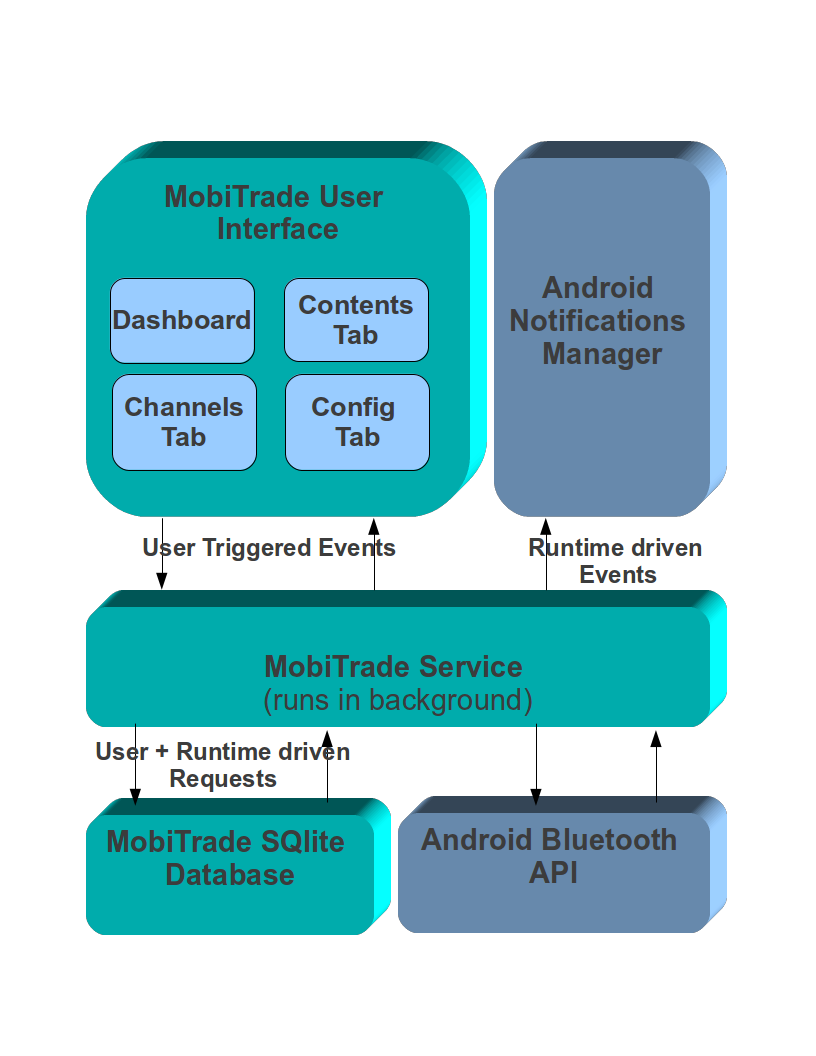
\includegraphics[width=3.5in,height=3in]{Chapitre6/MobiTradeCommunicationArchitecture.png}
\vspace{-0.1in}
\caption{MobiTrade Device Model}
\label{MobiTrade-application}
\vspace{-0.1in}
\end{figure}

Since MobiTrade is based on \emph{store-carry-and-forward} content sharing approach, nodes should be able to efficiently store channels records as well as their associated contents. Also, in the context of time/bandwidth limited contacts, MobiTrade application should also be able to identify and extract efficiently the list of contents that match a set of received channels records in order to answer the remote device upon a MobiTrade session. Convinced that the latter needs could be fully satisfied by a relational database engine and taking into consideration the fact that the selected engine should be supported by the our target platform (android), we choose to work with an SQLite database engine. Indeed, an SQLite~\cite{SQLite} database requires little or no administration, it is a good choice for devices or services that must work unattended and without human support. SQLite is a good fit for use in SmartPhones and it works very well as an embedded database in applications. So, as described in Figure~\ref{MobiTrade-application}, our MobiTrade mobile application uses and SQLite database engine for channels and contents records management.

With regards to the underlying wireless technology we choose to initially base our implementation on Bluetooth technology rather than on Wi-Fi but, we also intend to support the Wi-Fi in Ad-Hoc mode in the future. Indeed, the current android Java libraries do not support the ad-hoc mode of Wi-Fi although this is supported by both the driver and the hardware interface on almost android mobile devices. Therefore, making our implementation supporting the Ad-Hoc mode requires the device to be run in privileged user mode (i.e. rooted mode) so that the interface can be reconfigured to run in ad-hoc mode.

\subsection{MobiTrade Session}
\label{MobiTrade-session}

We mean by a MobiTrade session the protocol followed by a pair of mobile devices following a successful meeting and a wireless (Bluetooth) connection establishment. Figure~\ref{mobitradesession} depicts an UML (Unified Modeling Language) sequence diagram that describes in details the dynamics of a MobiTrade session between two devices $A$ and $B$. 

As described in Figure~\ref{mobitradesession}, the MobiTrade session is triggered by the device A that starts by serializing the channels records that it stores locally into an XML message (described in Figure~\ref{channelsxml}) then, it sends the serialized message throught the established Bluetooth channel towards the remote peer. Once received, the channels XML record is parsed within the device B using an XML SAX parser~\footnote{There are many XML parsers that are available. Choosing a right one for your situation might be challenging. Only three XML parsing techniques are extremely popular and are used for Java. Document Object Model (DOM), it is W3C provided mature standard, and Simple API for XML (SAX), it was one of the first to be widely adapted form of API for XML in Java and has become the standard, the third one is Streaming API for XML (StAX), which is a new model for parsing in XML but is very efficient and has a promising future. Each one of the mentioned techniques has their advantages and disadvantages. Choosing the right technique depends mainly on the application, its requirements and the hosting device capabilities. We choose to use a SAX parser since it is an event-driven parser that does not need to build the entire tree describing the XML document within memory and hence it does not require lot of memory space which is something we try to minimize within MobiTrade.}. The latter device extracts the channels attributes (keywords, utilities, ...) and decides based on them of the set of contents that could be of interest to the device A. Once the later contents are identified, MobiTrade schedules them based on the utilities of their matching channels and prepares them for forwarding upon a possible request from the TFT block. At the mean time, the device B serializes also its locally stored list of channels and sends them back to the device A. The latter follows the same steps as done by device B in order to identify any possible matching content. Once done, the MobiTrade protocol triggers the TFT algorithm within device A in order to run and manage the contents exchanging process. The TFT block serializes the first scheduled content into an XML message (described in Figure~\ref{contentxml}) and forwards the latter one to device B which in return will decide of the content to forward back based on the size of the received one. The TFT process continues until one of the devices or both of them exhaust their list of scheduled contents. 

\begin{figure}[!h]
\begin{center}
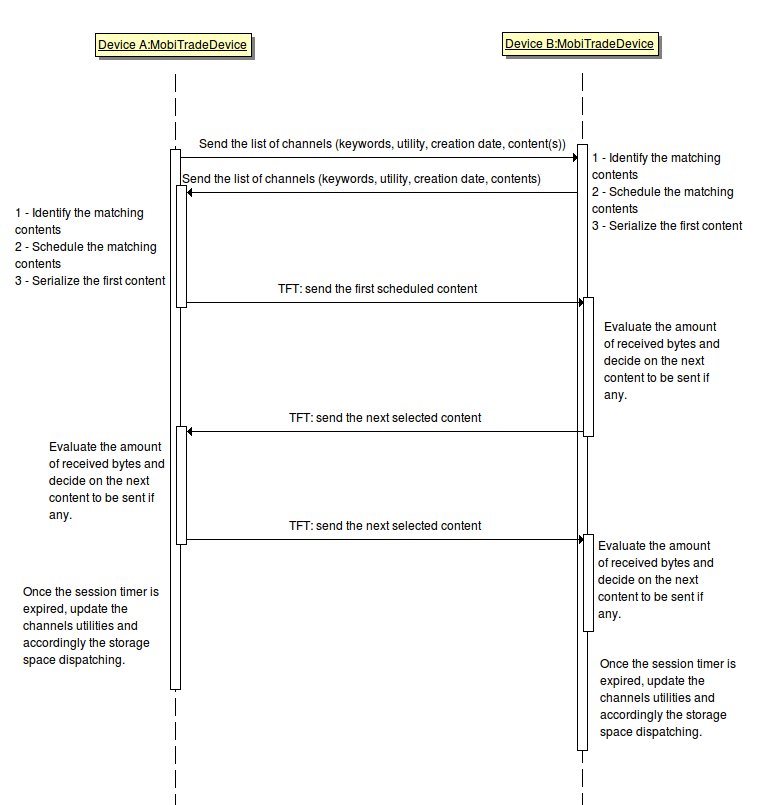
\includegraphics[width=5in,height=6in]{Chapitre6/MobiTradeSession.png}
\end{center}
\caption{MobiTrade session.}
\label{mobitradesession}
\end{figure}

\begin{figure}[!h]
\begin{center}
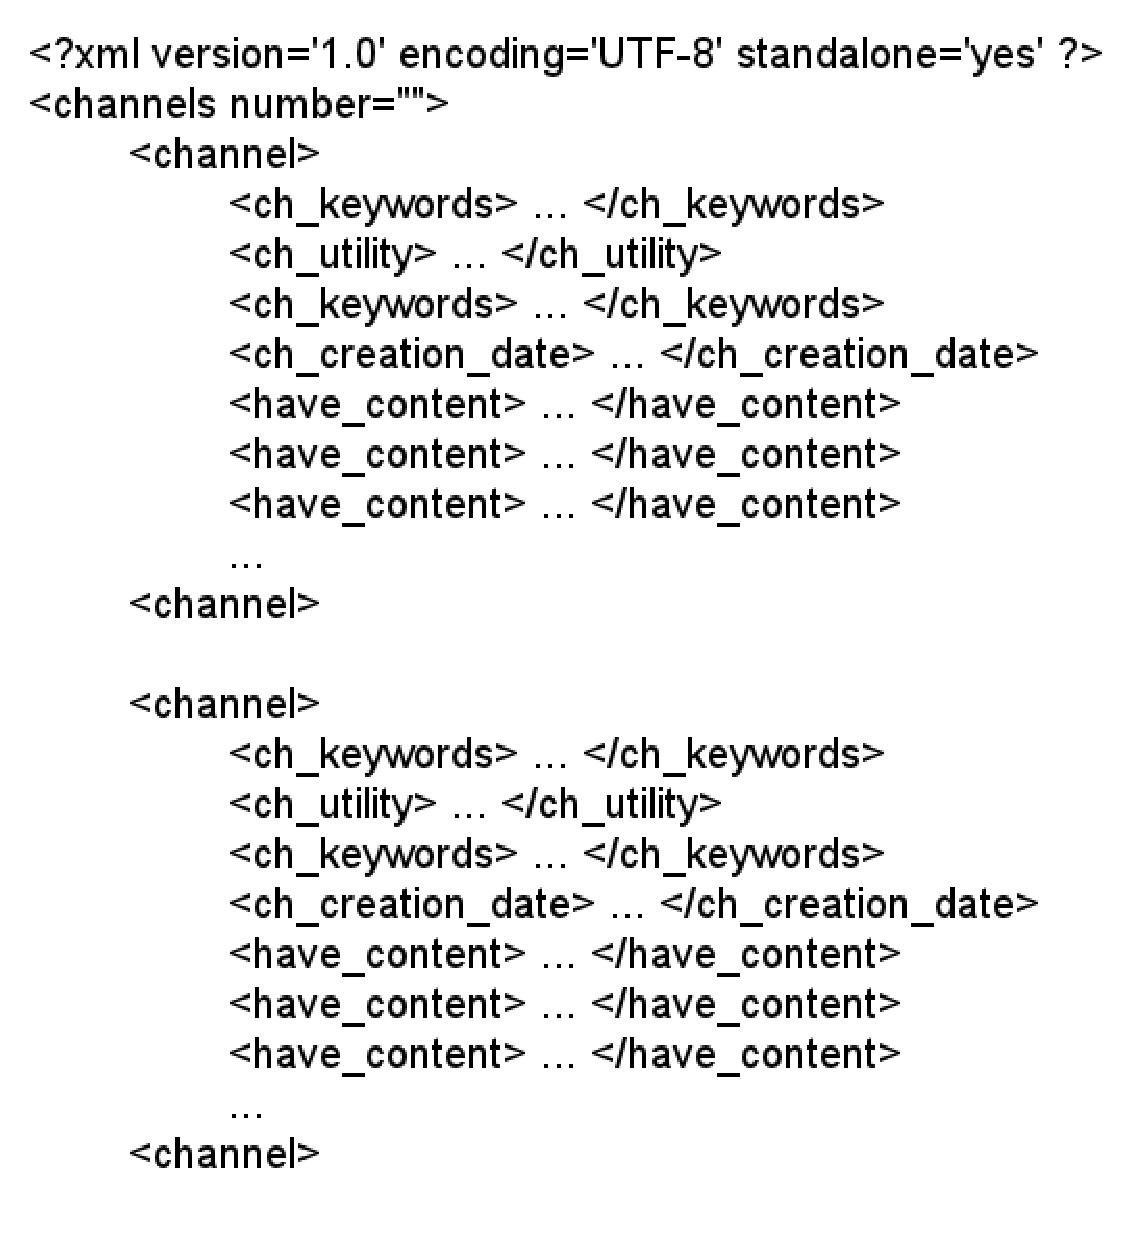
\includegraphics[width=4in,height=3in]{Chapitre6/channelsxml.eps}
\end{center}
\caption{Channels xml description .}
\label{channelsxml}
\end{figure}

Please note that in order to simplify the MobiTrade session and to make it as more efficient as possible, we choose to serialize also the content binary data within the XML document (see Figure~\ref{contentxml}). It is true that XML is not the ideal carrier for binary data. It is a text format, and as such doesn't cope well with raw bits. But, if binary data is properly encoded, using something like the W3C XML schema types Base64Binary, then using the XML converters reading and writing binary files becomes a snap. So, in our case, we use the Base-64 encoding/decoding format in order to be able respectively to include the content binary data as an element within the XML document (see Figure~\ref{contentxml}) at the sender side and to extract it at the receiver one.  

\begin{figure}[!h]
\begin{center}
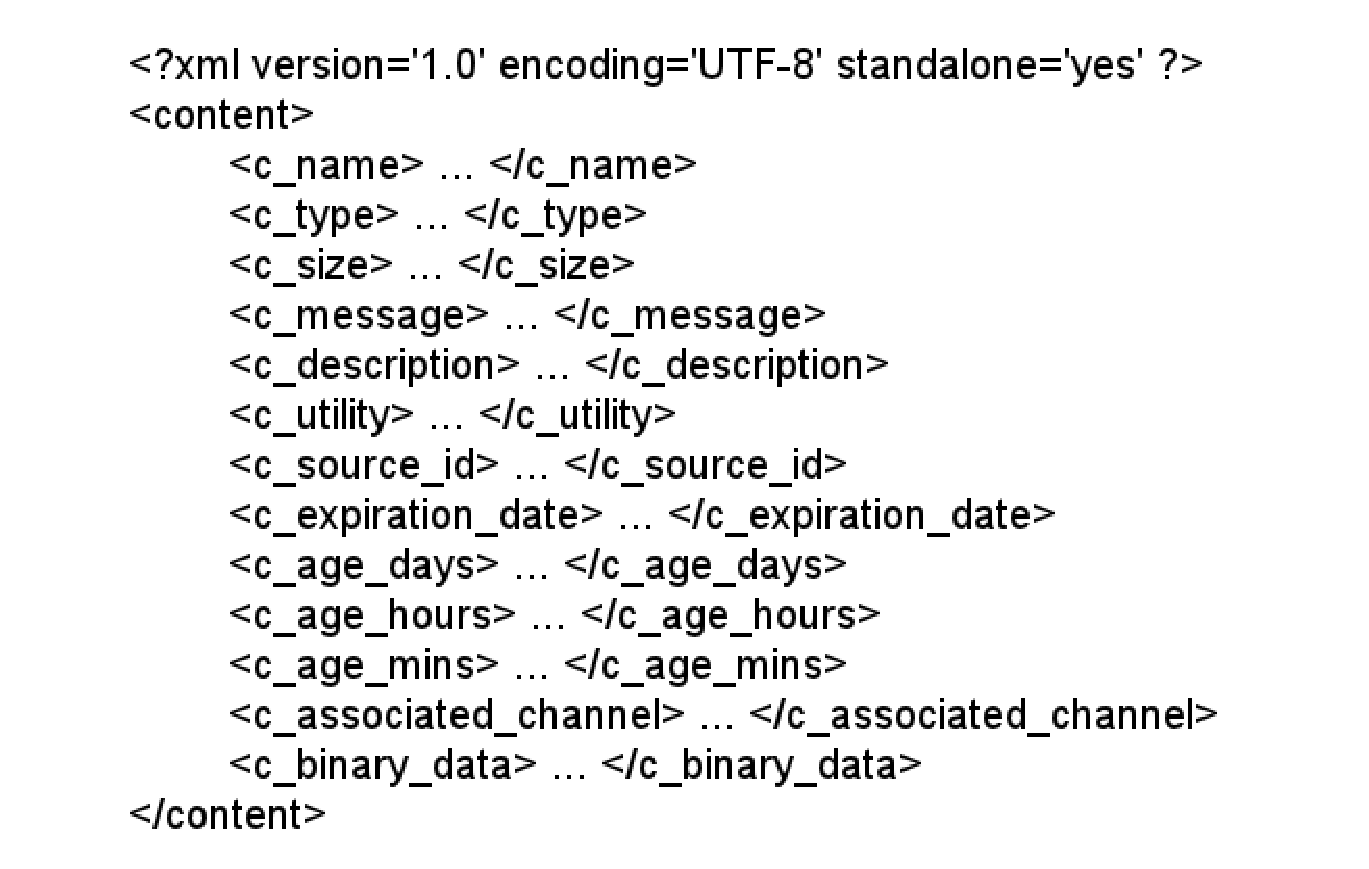
\includegraphics[width=4in,height=3in]{Chapitre6/contentxml.eps}
\end{center}
\caption{Content XML description.}
\label{contentxml}
\end{figure}






\section{MobiTrade Support for Bluetooth}
\label{MobiTradeDesignAndImplementation}

As explained before, we choose to initially base our implementation only on Bluetooth technology since the current android Java libraries do not support the ad-hoc mode of 802.11. Bluetooth is a low-power short-range wireless communication technology intended to replace the cables connecting electronic devices. Below we give a short overview on the Bluetooth protocol stack, the device discovery procedure (called inquiry scan in Bluetooth terminology), supported higher layer protocols and the application programming interfaces.

\subsection{Bluetooth Overview}

Bluetooth operates on a license-free ISM band at 2.4GHz (the same as used by 802.11). The physical layer is based on frequency hopping spread spectrum (FHSS) and transmits data on up to 79 frequency bands (1 MHz each). Each frequency band is divided into time slots and full duplex transmission is provided through the use of a time-division duplex (TDD) scheme.

Bluetooth network has a master-slave structure. A master device can communicate with up to seven devices forming a so called piconet. In a piconet devices communicate on the same physical channel that is defined by a common clock (set by the master) and a frequency hopping pattern. By definition, the device that initiates a connection becomes the master. Once a piconet has been established, master-slave roles may be exchanged. At any given time, data can be transferred between the master and one other device, but never directly between two slaves. A device can only be synchronized to a single channel at a time. Multiple simultaneous operations (e.g. partici-
pating in various piconets, being discoverable and connectable) are supported using time-division multiplexing between various channels. However, device can only be the master of a single piconet.

Above the physical layer in the architecture there is a number of logical links for control and data traffic. These are managed by a L2CAP layer that provides a channel based abstraction for applications. One logical (and physical) link can thus carry data for multiple applications. L2CAP provides reliable transmission performing flow control, CRC checks and retransmissions upon request. The main traffic services provided are asynchronous connection-oriented unicast and isochronous constant rate channel (e.g. for audio streaming). However, these channels are rarely used directly by applications, instead several higher layer protocols have been standardized and implemented in various client libraries. 

The most commonly adopted Bluetooth specifications include v1.2, v2.0 and v2.1 all being backwards compatible. The specifications differ mainly in supported bit rates and support for some advanced features. The nominal rate for Bluetooth v1.2 is 1Mbit/s. Bluetooth v2.0 increases the bit rate up to 2Mbit/s (Basic Rate) and 3Mbit/s (Enhanced Data Rate or EDR). v2.1 extends the inquiry responses (more on this below) and adds secure pairing among other minor tweaks. The operational ranges of Bluetooth devices vary from approximately 1, 10 to 100 meters (class 3, class 2 and class 1 respectively). Smartphones are generally class 2 devices.

\paragraph*{Inquery Scan Procedure}

The Bluetooth specification defines two separate physical channels for device discovery (inquiry scan channel) and connection setup (page scan channel).  Each Bluetooth devices can be in one of the four states: \emph{(1)} connectable and discoverable, \emph{(2)} connectable, \emph{(3)} discoverable, or \emph{(4)} neither discoverable nor connectable. A device cannot be discovered nor connected unless it is configured in the correct state.

A discoverable device listens for inquiry requests periodically (called inquiry scan state) on its inquiry scan channel that has a reduced number of hop frequencies and a slower rate of hopping. In order to discover neighboring devices, an inquiring device hops through all possible inquiry scan channel frequencies in a pseudo-random fashion, sending an inquiry request on each frequency and listening for responses. This is done at a faster rate, allowing the inquiring device to cover all inquiry scan frequencies in a reasonably short time period. The Bluetooth specification recommends an inquiry duration of 10.24s. Then, with high probability, all neighboring devices will
have entered their inquiry scan state and will hear the inquiry.

An inquiry response consists of an unique 48-bit device address of the discovered device and a 24-bit Class-of-Device code (CoD). The CoD consists of a major and minor device codes. The device codes are standardized and provide information about the device type: major code can tell if the device is a computer or a phone for example while the minor code can specify if the device is a cellular or cordless phone. In addition, each device may have a human readable name that can be queried using a separate control request. The extended inquiry response available in v2.1 can provided the human readable name and additional information about supported services directly in the inquiry response. Older Bluetooth devices must use the separate control request and a service discovery protocol (see below) instead.

Once a device is discovered, a connection setup can take place. A connectable device is listening on its page scan channel for connection requests that are send in a similar fashion as inquiry scans. The connection setup must be completed before any data can be transmitted between the devices.

\paragraph*{Higher Layer Protocols}

Each Bluetooth device must support the Service Discovery Protocol (SDP). The service discovery mechanism provides the means for client applications to discover the existence of services provided by server applications as well as the attributes of those services. The attributes of a service include the type or class of the service and the protocol information needed to access the service. The SDP protocol itself is run by a SDP server on the device that is responsible of maintaining the local service records and answering service discovery queries for SDP clients on other Bluetooth devices.

The Bluetooth specifications define various specialized protocols on top of the L2CAP layer for different purposes such as audio streaming, telephony and data transmissions. The most commonly used serial data stream protocol is RFCOMM. The RFCOMM protocol provides emulation of serial ports (up to 60 ports can be used simultaneously depending on the implementation). It provides a simple reliable data stream service, similar to TCP. In order to connect to another Bluetooth device over RFCOMM, the client must know the server channel which can be resolved using SDP. It is also possible to use hard-coded channels, but dynamic channel numbers are recommended since the number of available channels is very limited (30). 

Our MobiTrade android implementation makes use of the service discovery protocol (SDP) and and establishes an RFCOMM serial data stream in order to efficiently run a given MobiTrade session and to exchange the needed meta-data messagees as well as the contents themselves. According to MobiTrade architecture, each mobile device plays at the same time the role of a client and a server. So, it hosts a MobiTrade service which in return will accept and manage incomming connections and supports needed functionalities in order to initiate and run a MobiTrade session. Indeed,  using SDP, a MobiTrade device has the ability to identify wether the remote peer hosts a MobiTrade service or not. If a runnig service is discovered, then, the mobile device establishes an RFCOMM channel with the remote peer in order to exchange the needed messages.    

\paragraph*{Application Programming Interfaces}

The main interface between user level applications and the Bluetooth device is called Host Controller Interface (HCI) that is standardized in the Bluetooth specification. However, existing Bluetooth protocol stack implementations typically do not allow direct access to the HCI interface but provide their own abstractions of the main Bluetooth operations. The main stacks in use include BlueZ for Linux based devices 2, Windows Bluetooth stack and WinSock for Windows and Windows CE based devices 3 and Broadcom's Bluetooth stack for Windows based devices 4.

The client APIs let the applications control the device state (discoverable and/or connectable), the human readable Bluetooth device name and very often the CoD value. The device inquiry can be initiated at anytime through the Bluetooth API and the applications can typically control the duration of the inquiry and/or the number of responses to wait for. The applications can also query for the human readable names of the discovered devices, create local SDP records for the services they provide and query the records of nearby devices. The data services such as RFCOMM are typically accessed using a special type of socket and the familiar socket API.

\subsection{Android Platform Support for Bluetooth}

Since the android platform is based on a Linux kernel, the provided android Bluetooth API is nothing but a Java wrapper around the Linux BlueZ stack. These APIs let applications wirelessly connect to other Bluetooth devices, enabling point-to-point and multi-point wireless features. Using the Bluetooth APIs, an android application can perform the following:

\begin{itemize}
\item Scan for other Bluetooth devices
\item Query the local Bluetooth adapter for paired Bluetooth devices
\item Establish RFCOMM channels
\item Connect to other devices through service discovery
\item Transfer data to and from other devices
\item Manage multiple connections
\end{itemize}

More details about the android Bluetooth API that we used for the development of the MobiTrade application are provided in~\cite{AndroidBluetoothAPI}. 

\section{Functionalities provided by the MobiTrade Android Application}
\label{MobiTradeCurrentFunctionalities}

The current android implementation of MobiTrade provides to the user a simplified dashboard (see Figure~\ref{dashboard}) from which he can both follow and interact on real time with the MobiTrade service. Indeed, the user have access to the current device Bluetooth state (whether the adapter is on or off, whether it is in discoverable mode or not and whether the device is currently running a discovery session or not). A set of statistics are also presented within the dashboard like the total number of contents stored within the device, the \% of used space with respect to the total space allocated to the MobiTrade application, the total number of channels maintained within the system, how much among the latter ones the user requested locally and finally the number of Bluetooth discovered devices that run MobiTrade.
 
\begin{figure}[!h]
\begin{center}
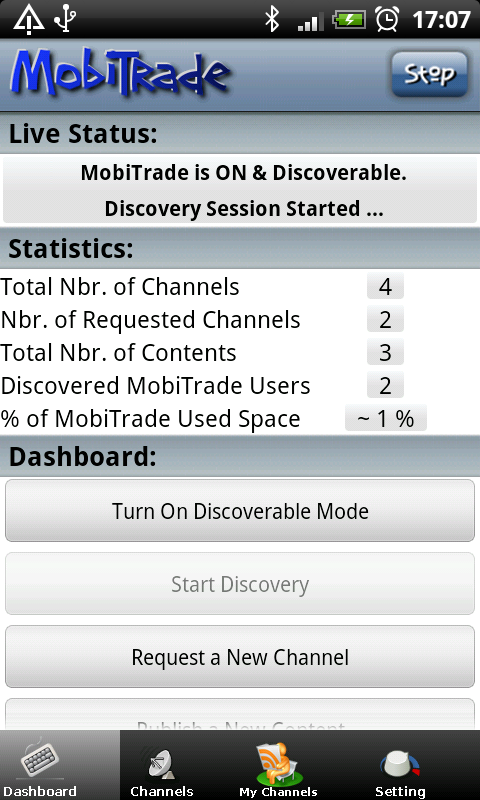
\includegraphics[width=2in,height=3in]{Chapitre6/Dashboard.png}
\end{center}
\caption{MobiTrade dashboard.}
\label{dashboard}
\end{figure}

In terms of functionalities, from within the dashboard depicted in Figure~\ref{dashboard}, the user is able to control the device Bluetooth discoverability, to control 
the Bluetooth discovery session, to manage channels (create new ones or join existing ones) and contents (create new contents or publish existing ones). We details in the following paragraphs the latter functionalities.

\paragraph{Bluetooth Interface Management}

One of the limitations that we faced along the implementation of MobiTrade was related to the android Bluetooth stack. Indeed, there
was no way to keep the mobile device discovrable to other non paired devices for more than 300 seconds. Enabling discoverability is necessary for MobiTrade to host a server socket that will accept incoming connections, because the remote non paired devices must be able to discover the device before it can initiate the connection. According to the android SDK, by default, enaibling discoverablity makes the device discoverable for $120$ seconds. The android SDK provides a way to define a different duration by adding the \emph{EXTRA\_DISCOVERABLE\_DURATION} Intent extra, however the maximum duration is fixed to 300 seconds.

In order to overcome the latter limitation, we have added a broadcast receiver to MobiTrade to catch android Bluetooth scan mode changements. Then, whenever the scan mode changes to not discoverable the user is notified, so he can decide wether to re-enable discoverability or not. This is could be done via the button \emph{"Turn On Discoverable Mode"} provided in the dashboard (see Figure~\ref{dashboard}).

Through the dashboard as well as the configuration tab described in Figure~\ref{Config}, we also provide to the user the control over the Bluetooth discovery sessions. Indeed, by default, whenever the MobiTrade service does not have a running content sharing session, it launches a Bluetooth discovery session trying to find new sharing opportunities. It is obvious that the latter behavior maximizes the probability of identifying new MobiTrade devices (sharing opportunities) however it can turn out very quickly to be a useless waste of energy (device battery). Indeed, if the user knows that he gonna be completely physically isolated from any possible sharing opportunity, he can decide to stop temporary the Bluetooth discovery session mechanism and event the Bluetooth adapter itself towards saving some energy then, restart everything later. To do this, the user should ask MobiTrade to give him back control over the Bluetooth discovery session mechanism by updating the corresponding entry in the configuration tab described in Figure~\ref{Config}. Then, the user can drive the discovery from within the dashboard (run it or stop it whenever needed).

\paragraph{Channels/Contents Management}

As describer in Chapter~\ref{chapter:PTMP}, MobiTrade manages autonomously the channels as well as their corresponding content records towards maximizing the revenues of the local user. At the same time, the current MobiTrade prototype provides to the user the possibility to interact and manage the set of locally stored channels/contents. Indeed, as described in Figure~\ref{JoiningNewChannel}, MobiTrade dashboard enables the user to ask for joining a new channel. The latter channel could be either an already discovered foreign channel (see Figure~\ref{JoiningExistingChannel} or a new channel that the user wants to create as depicted in Figure~\ref{CreatingNewChannel}.

\begin{figure}[!h]
\begin{minipage}[l]{0.3\linewidth}
\centering
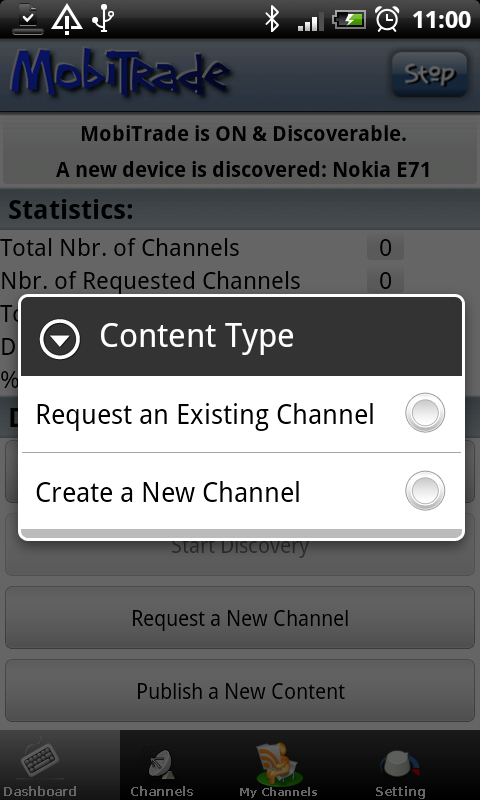
\includegraphics[width=2in,height=3in]{Chapitre6/JoinChannel.png}
\begin{minipage}[l]{1\linewidth}
\small
\caption{MobiTrade: Joining a new channel.}
\normalsize
\label{JoiningNewChannel}
\end{minipage}
\end{minipage}
\hspace{2.1cm}
\begin{minipage}[l]{0.3\linewidth}
\centering
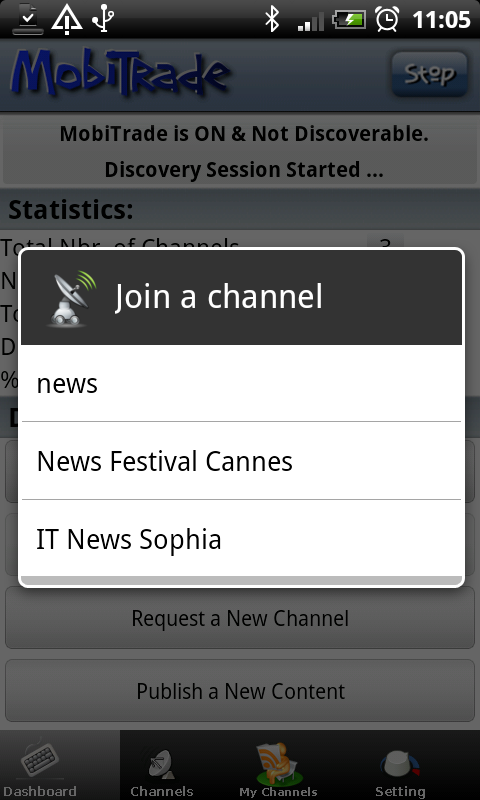
\includegraphics[width=2in,height=3in]{Chapitre6/JoinExistingChannel.png}
\begin{minipage}[l]{1\linewidth}
\caption{MobiTrade: Joining an existing channel.}
\label{JoiningExistingChannel}
\end{minipage}
\end{minipage}
\end{figure}

The channels tab described in Figure~\ref{ListAllChannels} enables the user to navigate through the available channels: the foreign channels that MobiTrade decided to collect and maintain locally for future trading as well as the locally requested ones. All the channel records are organized within a scrollable list which makes it easy for the user to navigate forward to the channels' corresponding contents (see Figure~\ref{ListAvailableContents}) and backward to the channels tab. Note that the locally requested channels are also presented apart in a separate tab (see Figure~\ref{ListRequestedChannels}) which we think provides a quick access to the channels of local interest and their matching contents.

\begin{figure}[!h]
\begin{minipage}[l]{0.3\linewidth}
\centering
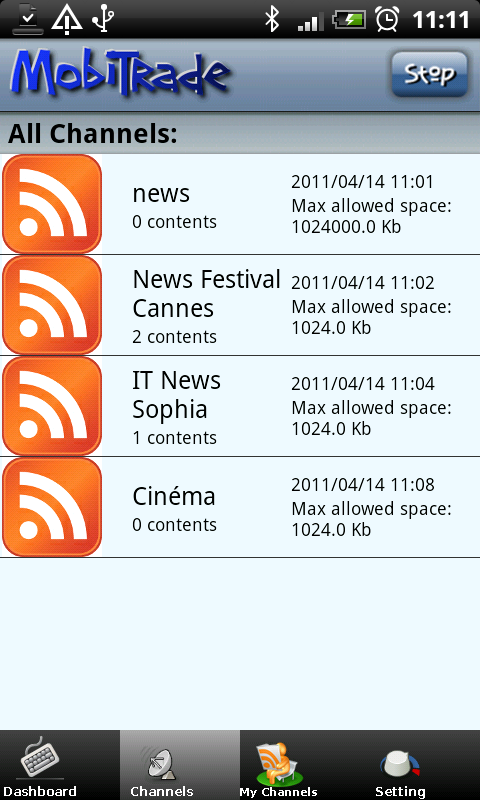
\includegraphics[width=2in,height=3in]{Chapitre6/ListAllChannels.png}
\begin{minipage}[l]{1\linewidth}
\small
\caption{MobiTrade: List of all channels.}
\normalsize
\label{ListAllChannels}
\end{minipage}
\end{minipage}
\hspace{2.1cm}
\begin{minipage}[l]{0.3\linewidth}
\centering
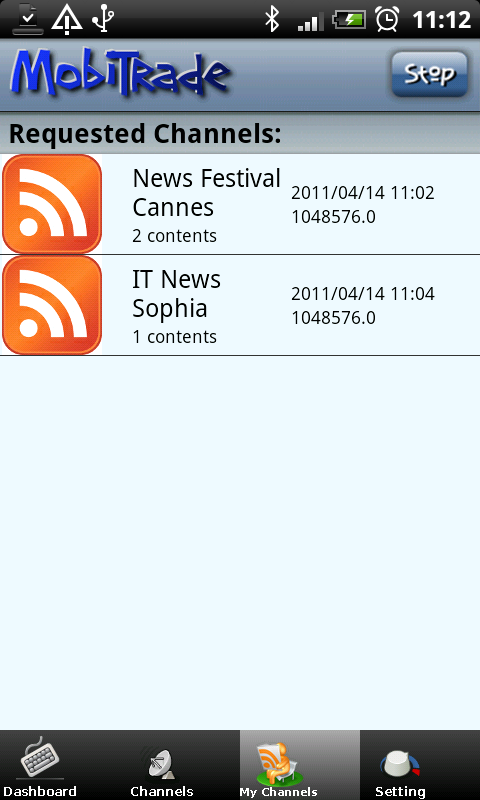
\includegraphics[width=2in,height=3in]{Chapitre6/ListRequestedChannels.png}
\begin{minipage}[l]{1\linewidth}
\caption{MobiTrade: List of locally requested channels.}
\label{ListRequestedChannels}
\end{minipage}
\end{minipage}
\end{figure}

From within the dashboard, the user is also able to publish a new content record. Once this task is initiated, the user is first asked to select the channel within which he wants to publish the new content. Then, as described in Figure~\ref{PublishNewContent}, the user can choose to either publish an existing content or crate a new one (see Figure~\ref{CreatingNewContent}) and in both case the user has to associate to the new content a short description which will be used later by MobiTrade to run the matching process between the content  and the channels records.

\begin{figure}[!h]
\begin{minipage}[l]{0.3\linewidth}
\centering
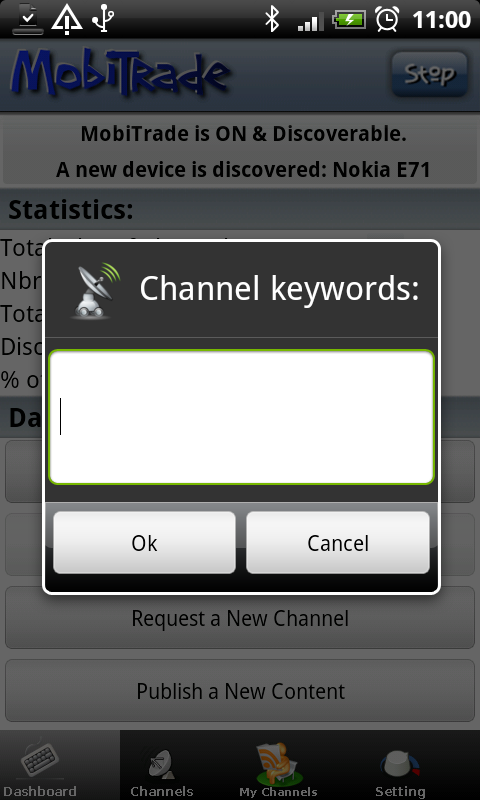
\includegraphics[width=2in,height=3in]{Chapitre6/CreateChannel.png}
\begin{minipage}[l]{1\linewidth}
\small
\caption{MobiTrade: Creating a new channel.}
\normalsize
\label{CreatingNewChannel}
\end{minipage}
\end{minipage}
\hspace{2.1cm}
\begin{minipage}[l]{0.3\linewidth}
\centering
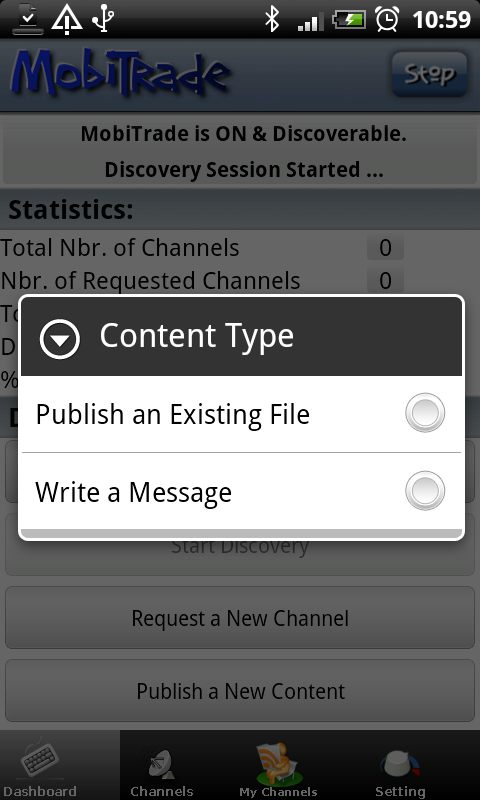
\includegraphics[width=2in,height=3in]{Chapitre6/PublishContent.png}
\begin{minipage}[l]{1\linewidth}
\caption{MobiTrade: Publishing a new content.}
\label{PublishNewContent}
\end{minipage}
\end{minipage}
\end{figure}


\begin{figure}[!h]
\begin{minipage}[l]{0.3\linewidth}
\centering
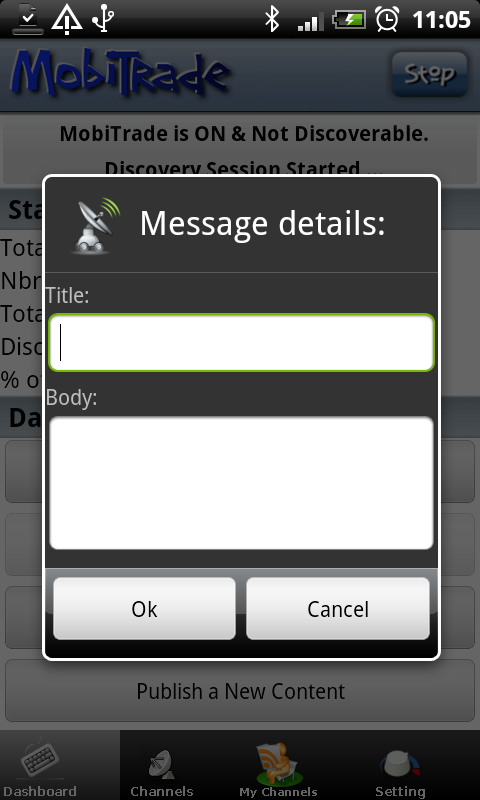
\includegraphics[width=2in,height=3in]{Chapitre6/WriteMessage.png}
\begin{minipage}[l]{1\linewidth}
\small
\caption{MobiTrade: Creating a new content/message.}
\normalsize
\label{CreatingNewContent}
\end{minipage}
\end{minipage}
\hspace{2.1cm}
\begin{minipage}[l]{0.3\linewidth}
\centering
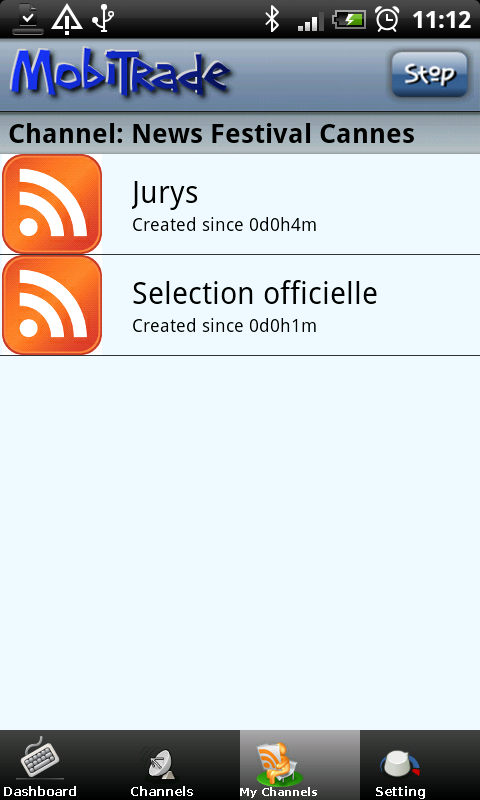
\includegraphics[width=2in,height=3in]{Chapitre6/ListContents.png}
\begin{minipage}[l]{1\linewidth}
\caption{MobiTrade: List of available contents with respect to the selected channel.}
\label{ListAvailableContents}
\end{minipage}
\end{minipage}
\end{figure}

\paragraph{MobiTrade Configuration}

As described in Figure~\ref{Config}, MobiTrade configuration tab provides to the user the possibility to tune some important parameters within the MobiTrade architecture. 

Namely, towards controlling the device resources usage (both local storage as well as battery), first  \emph{(i)} it is made possible for the user to specify the maximum amount of storage space that MobiTrade is allowed to use both for storing locally requested contents as well as contents used for trading. And second \emph{(ii)}, as described above in this section, the user can either leverage the control of the Bluetooth discovery sessions to MobiTrade service which will try to keep always discovering new sharing opportunities or he can take the control over that process and decide on the moment at which the device should run a discovery session. Following the latter option, the user can save lot of battery power without loosing in terms of expected revenues from possible sharing opportunities.

Through the Configuration tab, the user also have the possibility the specify whether he wants or not to get notified via the device vibrator (if supported) whenever a new content that matches a locally requested channel is received. Indeed, this is a very interesting option because the user is not supposed to keep tracking on real-time the status of the content sharing sessions. Instead, the user can start MobiTrade service, choose to get notified, then close the MobiTrade UI and head out on the real world. Then, whenever a new content of interest is received, the user will be notified. Note that the MobiTrade UI is completely decoupled from the MobiTrade service in terms of \emph{life cycle}. MobiTrade UI could be down and at the same time MobiTrade service is running in background. And any time the user launches the MobiTrade activity (UI), he can control/follow on real from within the dashboard what is going on with the MobiTrade service.

Note that MobiTrade configuration is maintained persistently within the mobile device. Thus, each time the user decides to update one of the configuration entries, he should validate the new configuration from within the tab. There will be always the possibility to re-load default configuration entries.

\begin{figure}[!h]
\begin{center}
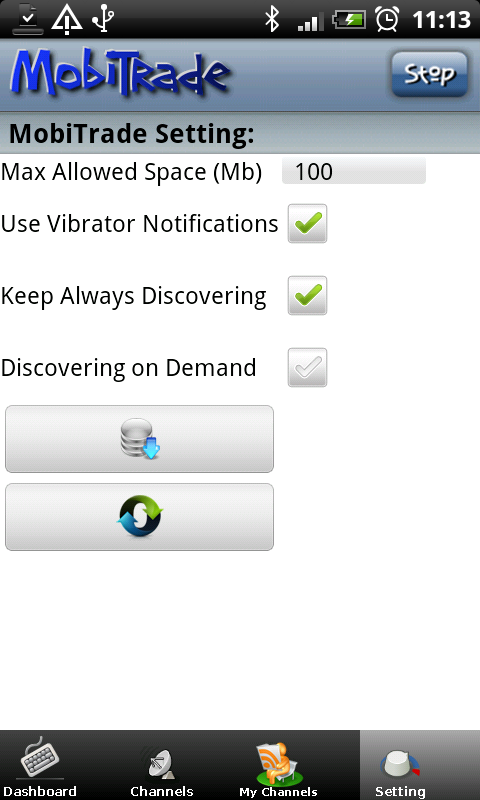
\includegraphics[width=2in,height=3in]{Chapitre6/Config.png}
\end{center}
\caption{MobiTrade: Configuring the daemon.}
\label{Config}
\end{figure}

\section{Summary and Open Issues}
\label{MobiTradeSoftSummary}

We have described the design and implementation of our architecture for the Google android platform. Our experience from the implementation is that android is a very powerful platform and quite mature. The Java based environment provides a familiar environment with good support for most common OS primitives such as threads and concurrency, database and content storage and inter process communication through the android service binding mechanism. Some features are however still missing, in particular support for the 802.11 ad-hoc mode (which needs to be implemented in native code). We believe that our design is general and facilitates the implementation of 
advanced content-centric applications. There are however some issues that are not, or only partially addressed by our design. We do currently not address particularly the issues of privacy, security and power management.
